\documentclass[8pt]{beamer}

% Der Plan
% Folie 1: Introduction: Henry
% Folie 2: Dataset: Christopher
% Folie 3: Network Architecture: Christopher
% Folie 4: Hyperparameter: Christopher
% Folie 5: Overtraining: Christopher
% Folie 6: Results: Henry
% Folie 7: Alternative Methods: Henry
% Folie 8: Conclusion: Henry
% Appendix: ???

% unverzichtbare Mathe-Befehle
\usepackage{amsmath}
% viele Mathe-Symbole
\usepackage{amssymb}
% Erweiterungen für amsmath
\usepackage{mathtools}

% Fonteinstellungen
\usepackage{fontspec}
% Latin Modern Fonts werden automatisch geladen

% deutsche Spracheinstellungen
% \usepackage[ngerman]{babel}
\usepackage[english]{babel}
%BUG in Biblatex wird hiermit gefixt
\providetoggle{blx@lang@captions@english}

\usepackage[
  math-style=ISO,    % ┐
  bold-style=ISO,    % │
  sans-style=italic, % │ ISO-Standard folgen
  nabla=upright,     % │
  partial=upright,   % ┘
  warnings-off={           % ┐
    mathtools-colon,       % │ unnötige Warnungen ausschalten
    mathtools-overbracket, % │
  },                       % ┘
]{unicode-math}

% traditionelle Fonts für Mathematik
\setmathfont{Latin Modern Math}
\setmathfont{XITS Math}[range={scr, bfscr}]
\setmathfont{XITS Math}[range={cal, bfcal}, StylisticSet=1]

% Zahlen und Einheiten
\usepackage[
  % locale=DE,                   % deutsche Einstellungen
  locale=US,
  separate-uncertainty=true,   % immer Fehler mit \pm
  per-mode=symbol-or-fraction, % / in inline math, fraction in display math
]{siunitx}

% richtige Anführungszeichen
\usepackage[autostyle]{csquotes}

% schöne Brüche im Text
\usepackage{xfrac}

% Grafiken können eingebunden werden
\usepackage{graphicx}

% Grafiken können in LaTex gemalt werden
\usepackage{tikz, pgfplots}

% Ermöglicht relative Positionierung von tikz-Nodes
\usetikzlibrary{positioning}

% Für Feynman-Graphen mit Tikz
\usepackage{feynmp-auto}

% Für komplexere Captions
\usepackage{caption}

% Für URL-Formatierung
\usepackage{url}

% Für Tabellen
\usepackage{booktabs}

% Literaturverzeichnis
\usepackage[
  backend=biber,
  style=authoryear,
  autocite=inline,
]{biblatex}
% Quellendatenbank
\addbibresource{presentation.bib}

\usetheme[numbering=fraction]{metropolis}

% Für die Titelseite
%\title{The Influence of Music Genres on Performance Metrics: A Comparative Analysis of Spotify and YouTube}
\title{The Genre Factor}
\subtitle{Project Presentation - ML Seminar 2023}
\author{Henry Krämerkämper\\%
  \and%
  Christopher Breitfeld}
\institute{Technische Universität Dortmund}
\date{13.07.2023}
\logo{
\includegraphics[height=0.5cm]{figures/tu_logo_sw_klein.pdf}}

\begin{document}

\begin{frame}
  \titlepage
\end{frame}

\begin{frame}
\frametitle{Introduction to the Problem}
  \begin{columns}
  \column{0.5\textwidth}
    \begin{itemize}
      \item Genre classification of songs based on the tracks features
      \item Dataset: Thousands of songs with diverse genres
      \item Challenge: Developing an accurate classification model
    \end{itemize}
  \column{0.5\textwidth}
  \tiny
  \begin{tabular}{l l}
    \toprule
    $\text{Feature}$ & $\text{Value}$ \\
    \midrule
    Artist & Gorillaz \\
    Url\_spotify & \url{https://open.spotify...} \\
    Track & Feel Good Inc. \\
    Album & Demon Days \\
    Album\_type & album \\
    Uri & spotify:track:0d28khcov6AiegS... \\
    Danceability & 0.818 \\
    Energy & 0.705 \\
    Key & 6.0 \\
    Loudness & -6.679 \\
    Speechiness & 0.177 \\
    Acousticness & 0.00836 \\
    Instrumentalness & 0.00233 \\
    Liveness & 0.613 \\
    Valence & 0.772 \\
    Tempo & 138.559 \\
    Duration\_ms & 222640.0 \\
    Url\_youtube & \url{https://www.youtube...} \\
    Title & Gorillaz - Feel Good Inc. (Official... \\
    Channel & Gorillaz \\
    Views & 693555221.0 \\
    Likes & 6220896.0 \\
    Comments & 169907.0 \\
    Description & Official HD Video for Gorillaz'... \\
    Licensed & True \\
    official\_video & True \\
    Stream & 1040234854.0 \\
    \bottomrule
  \end{tabular}
  \end{columns}
  \normalsize
\end{frame}

\begin{frame}
  \frametitle{Description of the Data Set}
    \begin{alertblock}{Dataset from \href{https://www.kaggle.com/datasets/salvatorerastelli/spotify-and-youtube}{Kaggle}: Spotify and YouTube}
      \begin{itemize}
        \item Contains statistics of $\SI{20.7}{\kilo}$ songs on Spotify and YouTube
        \item Does \alert{NOT} include genre information.
      \end{itemize}
    \end{alertblock}
    \begin{alertblock}{Wikidata Query for the Top-Genre of the Artist}
      \begin{itemize}
       \item Query artist’s Wikidata page for genres
       \item Assign artists/album genre to song
      \end{itemize}
    \end{alertblock}
    \vspace*{-0.5cm}
    \begin{columns}[t]
        \begin{column}{0.1\textwidth}
        \end{column}
        \begin{column}{0.3\textwidth}
            \begin{alertblock}{Selection}
                \begin{itemize}
                    \item Group Subgenres into Supercategories
                    \item Select sample of $\num{6}$ Genres
                    \item Remaining Songs: $\num{6446}$
                \end{itemize}
            \end{alertblock}
        \end{column}
        \begin{column}{0.7\textwidth}
            \begin{figure}
%                \hspace*{-0.8cm}
                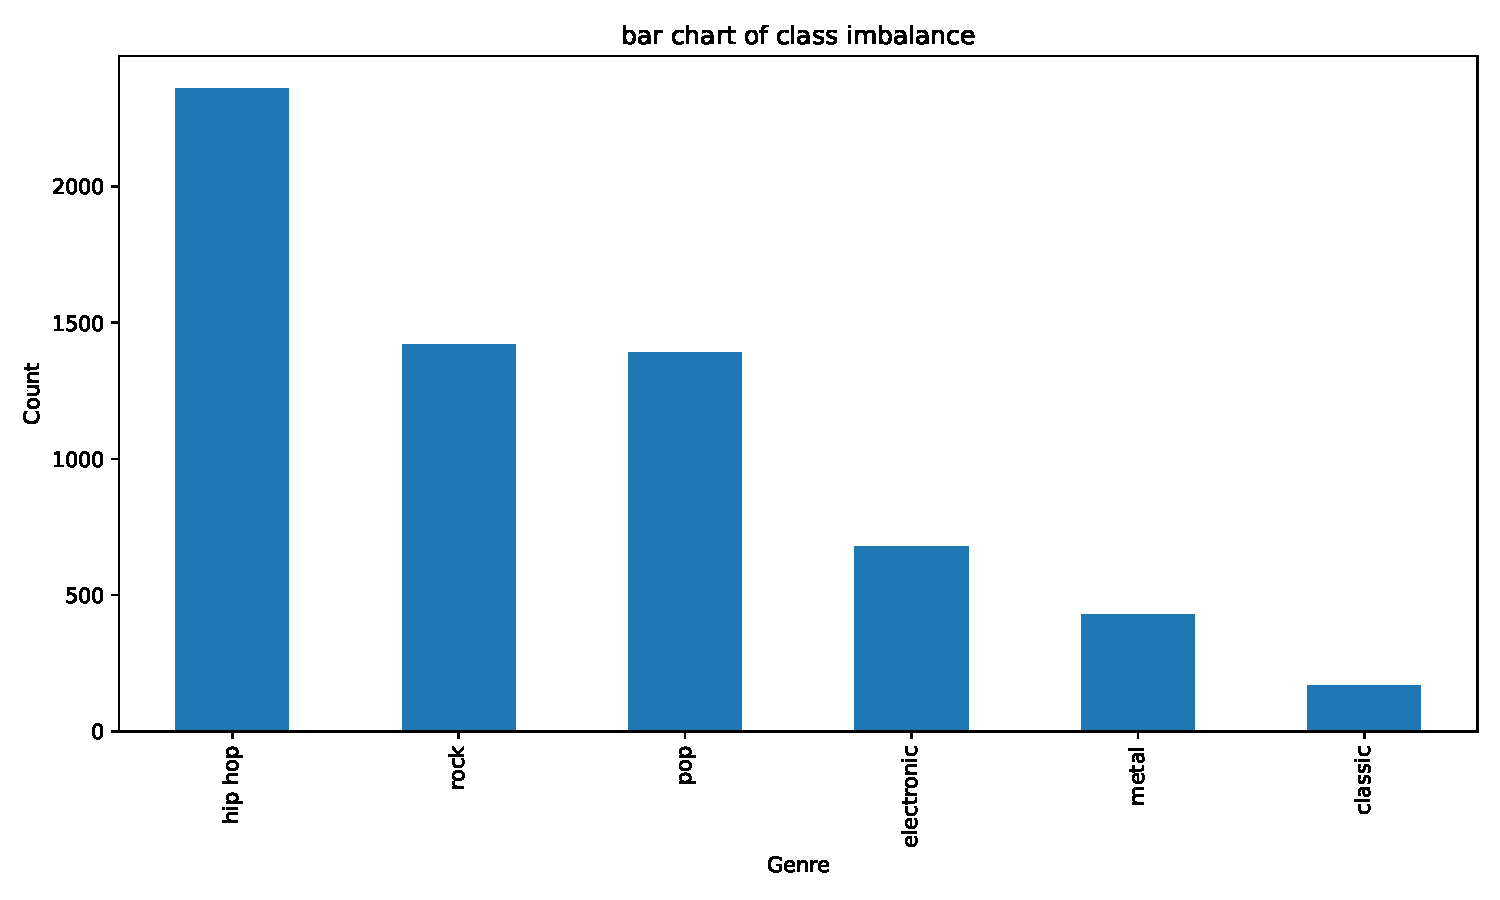
\includegraphics[width=\textwidth]{figures/genre_hist.pdf}
            \end{figure}
        \end{column}
    \end{columns}
\end{frame}

\begin{frame}
    \frametitle{Network Architecture}
    \begin{columns}[T]
        \begin{column}{0.7\textwidth}
            \begin{alertblock}{Model}
                \begin{itemize}
                    \item $\num{4}$ Dense Layers with Dropout
                    \item Trainable parameters: $\num{170246}$
                    \item Loss function: categorical crossentropy
                    \item Optimizer: adam
                \end{itemize}
            \end{alertblock}
            \begin{alertblock}{Training}
                \begin{itemize}
                    \item Early stopping: Stops training when the validation loss function no longer improves
                    \item Reduce learning rate: Decreases learning rate if validation loss function stagnates \\
                    \to better convergence
                    \item Train the model using the training data with the defined set of hyperparameters.
                \end{itemize}
            \end{alertblock}
        \end{column}
        \begin{column}{0.3\textwidth}
            \begin{tikzpicture}[
                scale=0.8, every node/.style={scale=0.8},
                layer/.style={rectangle,draw=black,fill=blue!30,minimum size=1cm},
                sum/.style={circle,draw=black,fill=yellow!30},
            ]

            % Define nodes
            \node[layer] (L0) at (0,0) {Input};
            \node[layer] (L1) at (0,-2) {\begin{tabular}{c} Dense (128) \\ Dropout (0.3) \end{tabular}};
            \node[layer] (L2) at (0,-4) {\begin{tabular}{c} Dense (256) \\ Dropout (0.3) \end{tabular}};
            \node[layer] (L3) at (0,-6) {\begin{tabular}{c} Dense (512) \\ Dropout (0.3) \end{tabular}};
            \node[layer] (L4) at (0,-8) {Dense (6)};

            % Draw connections
            \draw[->] (L0) -- (L1);
            \draw[->] (L1) -- (L2);
            \draw[->] (L2) -- (L3);
            \draw[->] (L3) -- (L4);

            % Draw parameter counts
            \draw (L0) -- (L1) node[midway,right] {2560 params};
            \draw (L1) -- (L2) node[midway,right] {33024 params};
            \draw (L2) -- (L3) node[midway,right] {131584 params};
            \draw (L3) -- (L4) node[midway,right] {3078 params};

            \end{tikzpicture}
        \end{column}
    \end{columns}

\end{frame}

\begin{frame}
    \frametitle{Hyperparameter Optimization}
    \begin{alertblock}{Method}
        \begin{itemize}
            \item Grid Search: Train models with all combinations of hyperparameters
        \end{itemize}
    \end{alertblock}
    \begin{alertblock}{Validation}
        \begin{itemize}
            \item $k=\num{3}$ Cross Validation
            \item Save train/validation Accuracy and Loss
        \end{itemize}
    \end{alertblock}
    \begin{figure}
        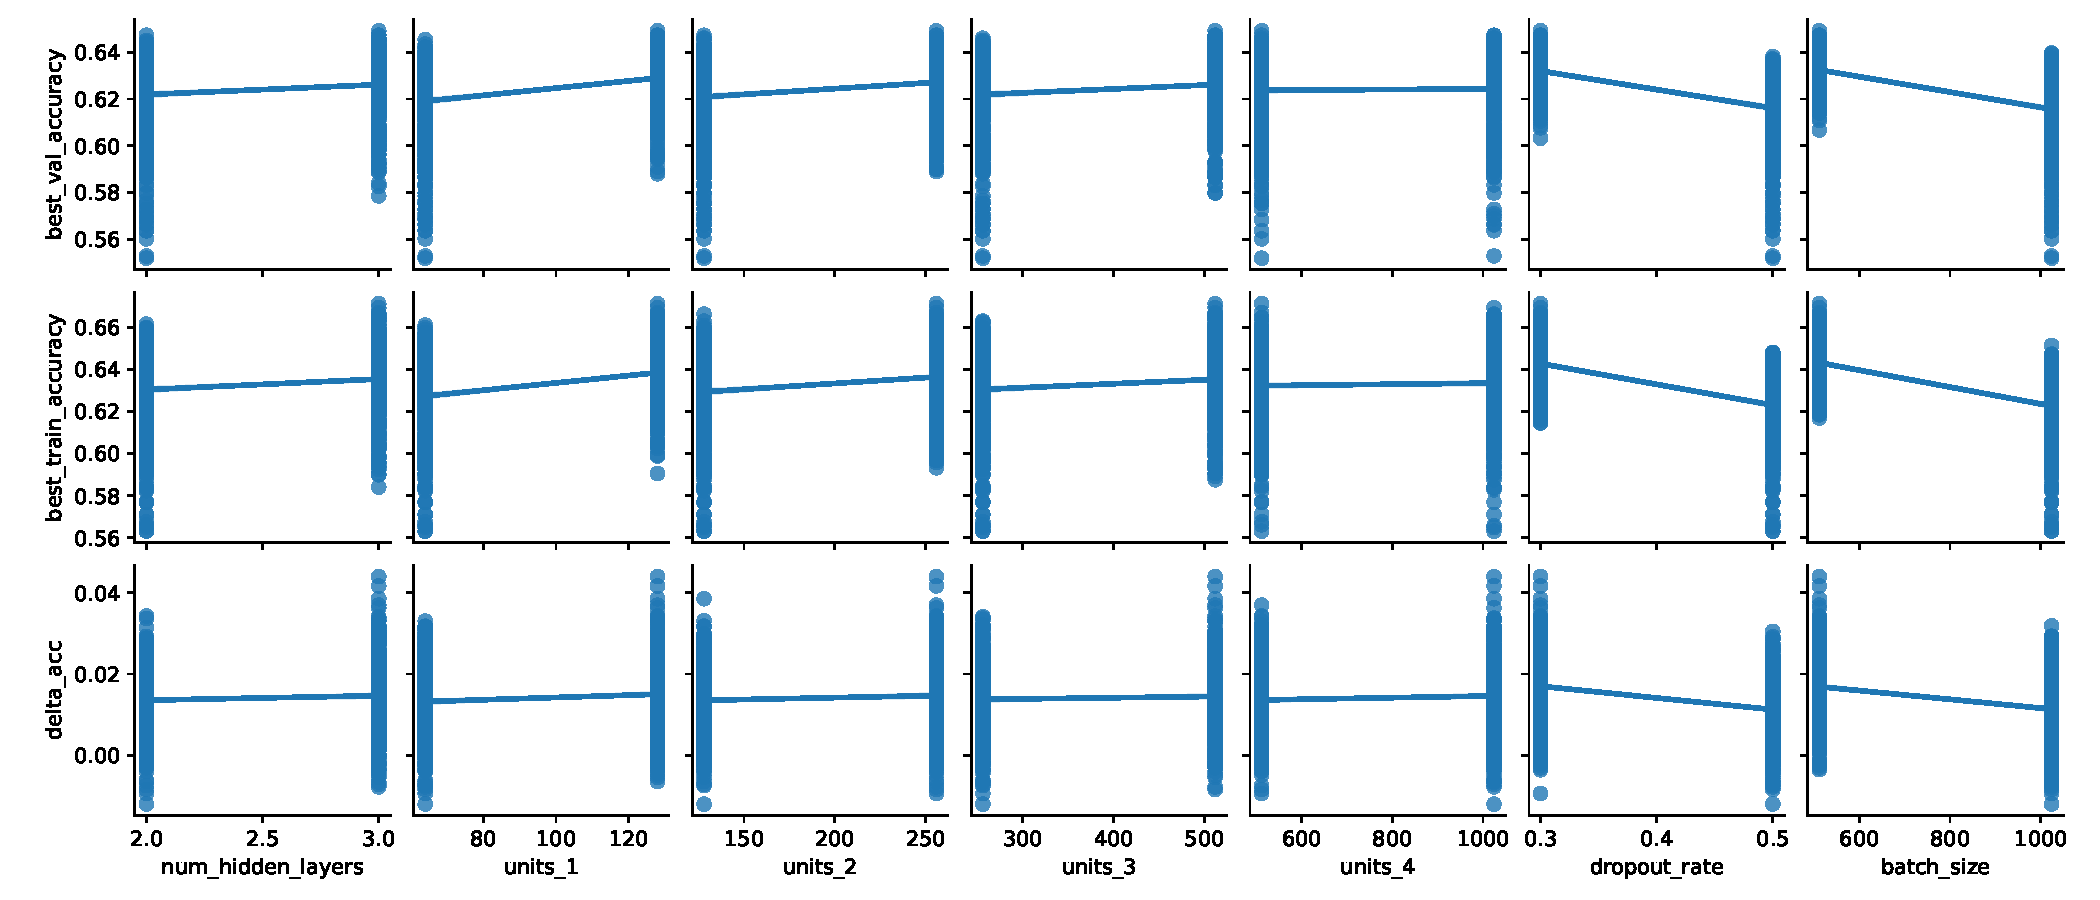
\includegraphics[scale=0.3]{figures/HPO_parameter.pdf}
    \end{figure}
\end{frame}

\begin{frame}
    \frametitle{Overtraining Checks}
    \begin{alertblock}{Methods to prevent Overtraining}
        \begin{itemize}
            \item Dropout
            \item Early stopping
            \item Minimize (Training Acc. - Validation Acc.)
            \alert{but} maximize Validation Acc.
        \end{itemize}
    Try different values and decide after Hyperparameter Optimization
    \end{alertblock}
    \begin{figure}
        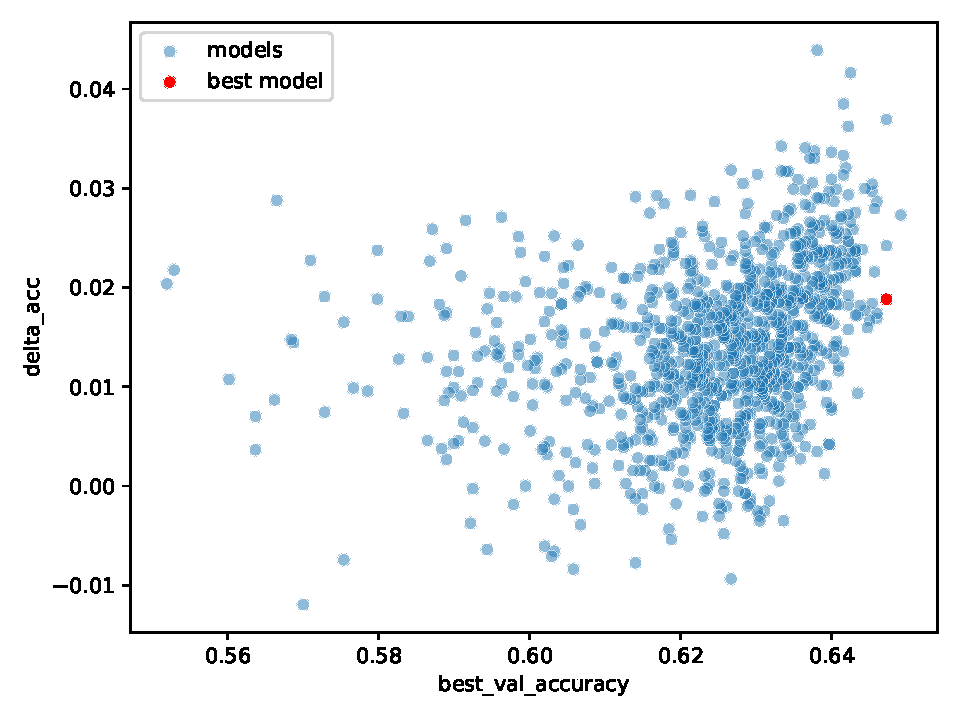
\includegraphics[scale=0.45]{figures/HPO_scatter.pdf}
    \end{figure}
\end{frame}

\begin{frame}
\frametitle{Results of our Neural Network}
\only<1>{
\begin{alertblock}{Accuracy and AUC-PR}
	\begin{itemize}
   \item Results in an accuracy of $\SI{65.56}{\percent}$ on test data
   \item As well as an AUC-PR score of $\num{0.738}$
  \end{itemize}
\end{alertblock}
    \begin{figure}
        \begin{minipage}[b]{0.48\textwidth}
            \centering
            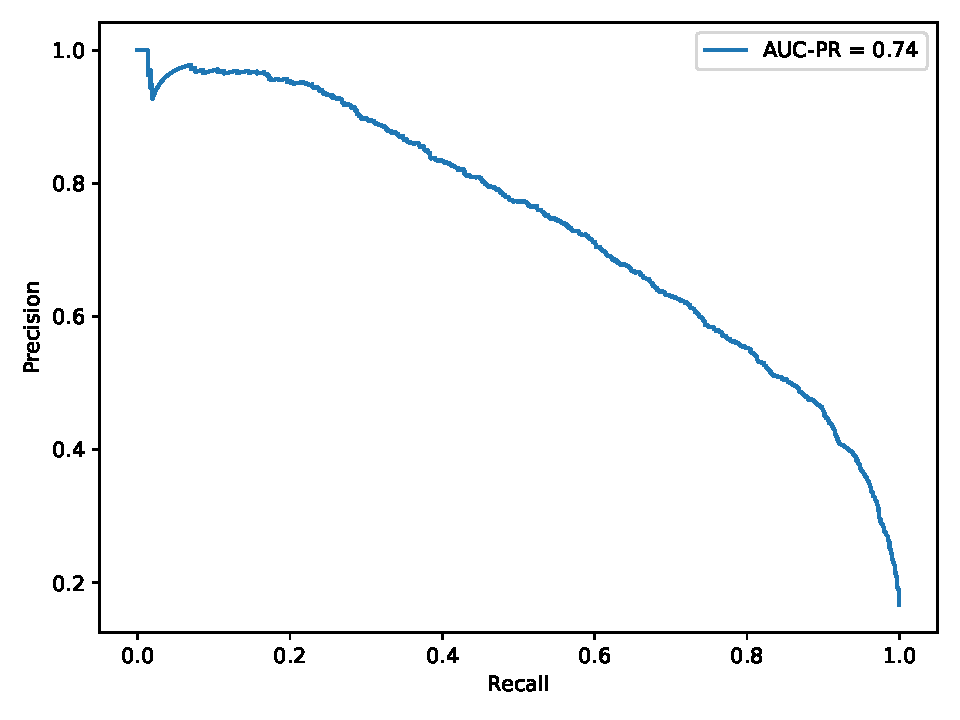
\includegraphics[width=\textwidth]{figures/PR_curve.pdf}
        \end{minipage}
        \hfill
        \begin{minipage}[b]{0.48\textwidth}
            \centering
            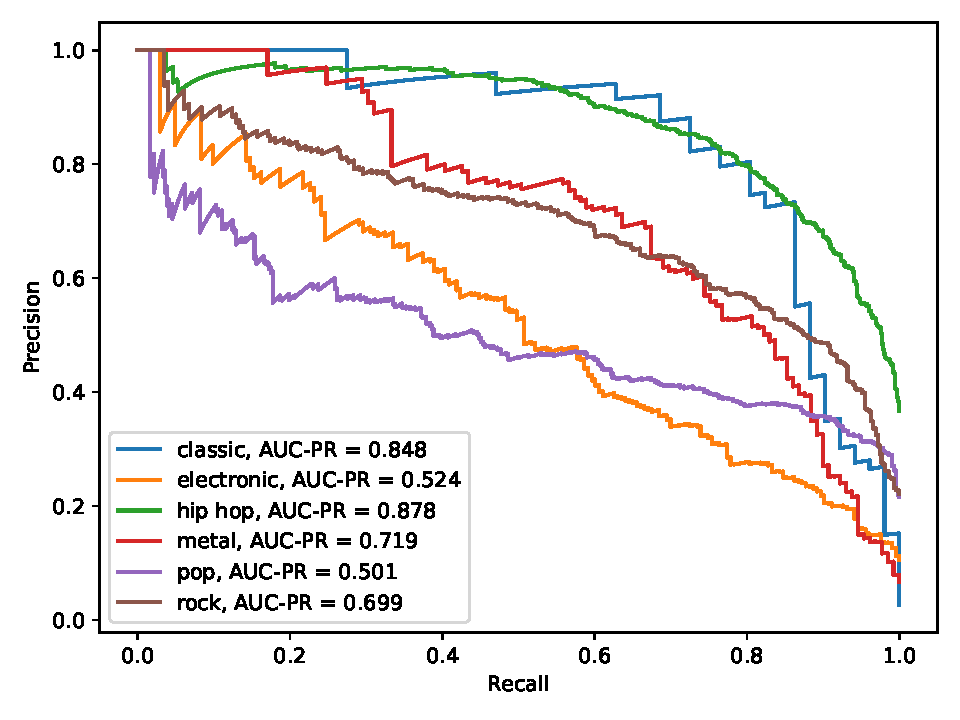
\includegraphics[width=\textwidth]{figures/PR_curve_genres.pdf}
        \end{minipage}
    \end{figure}
}
\only<2>{
\begin{figure}
  \centering
  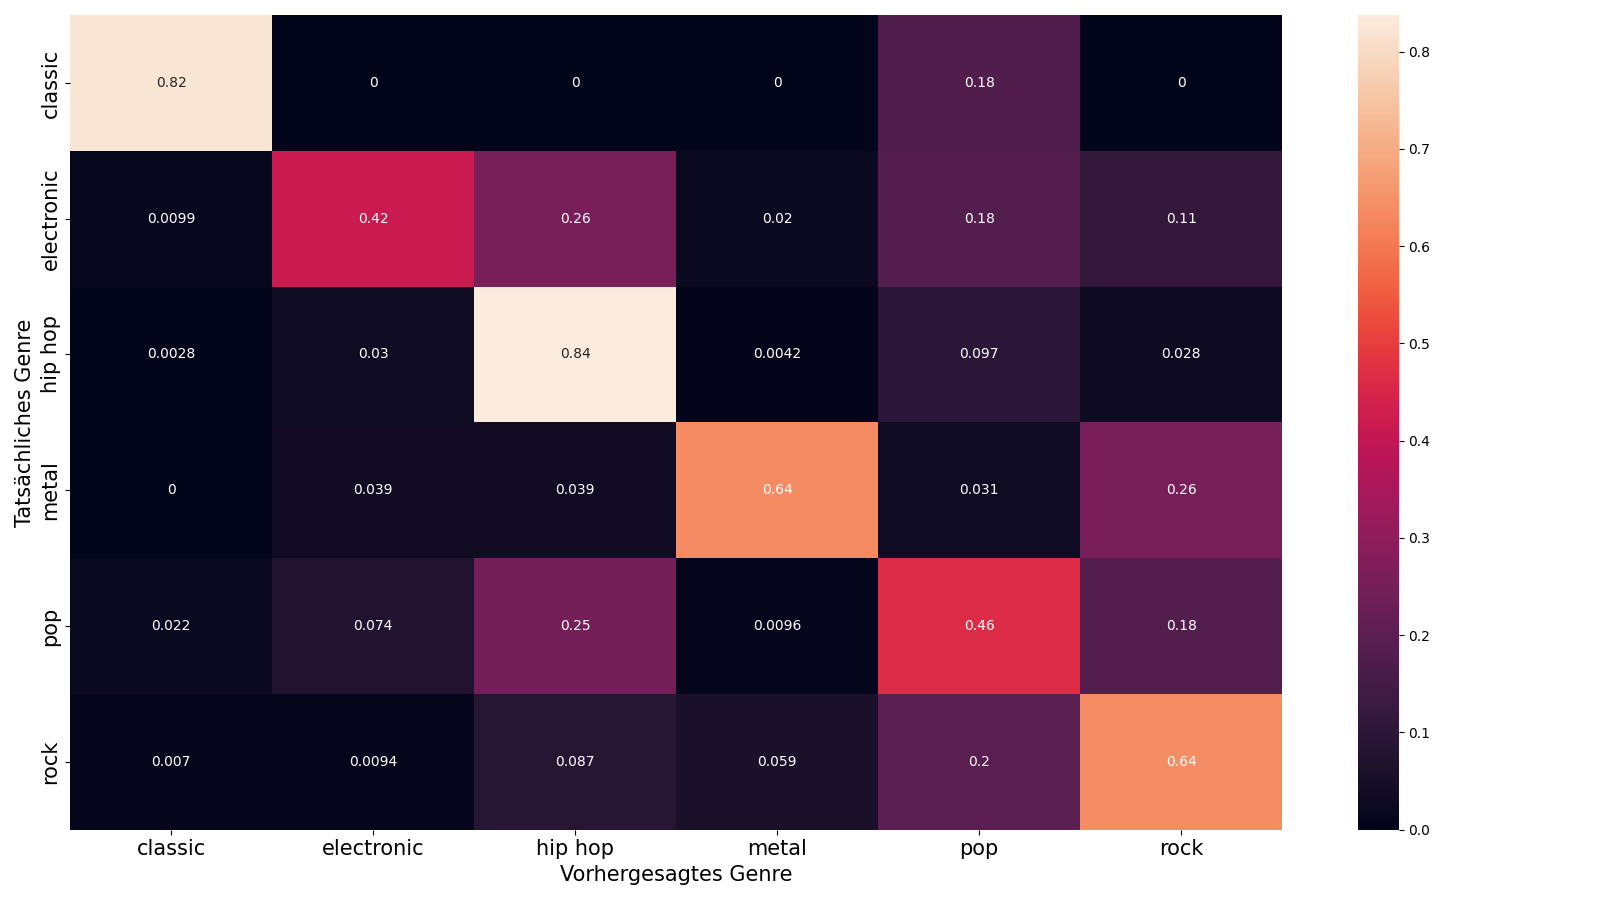
\includegraphics[scale=0.32]{figures/confusion_matrix_NN.png}
\end{figure}
}
\end{frame}

\begin{frame}
\frametitle{Alternative Methods}
  \begin{alertblock}{K-nearest-neighbors}
    \begin{itemize}
     \item Use $k=12$ as it achieves the highest performance
     \item Results in an accuracy of $\SI{60.62}{\percent}$
    \end{itemize}
  \end{alertblock}
  \begin{alertblock}{Support vector machines}
    \begin{itemize}
    \item{Model that classifies data by finding the hyperplane that maximally separates different categories in a multidimensional space}
    \item Use an One-vs-One approach to be able to do Multiclass-Classification:
    \begin{itemize}
      \item A separate model is trained for each pair of classes, and a given data point is classified by majority voting among the classifiers
      \end{itemize}
    \item The used kernel function is the radial basis function (RBF)
    \item Results in an accuracy of $\SI{63.88}{\percent}$
    \end{itemize}
  \end{alertblock}
\end{frame}

\begin{frame}
\frametitle{Conclusions}
  \begin{itemize}
          \item NN achieves an accuracy of $\SI{65.56}{\percent}$ on test data.
          \item Diminishing returns for more complex models, we are constrained by the dataset
  \end{itemize}
  \begin{figure}
    \centering
    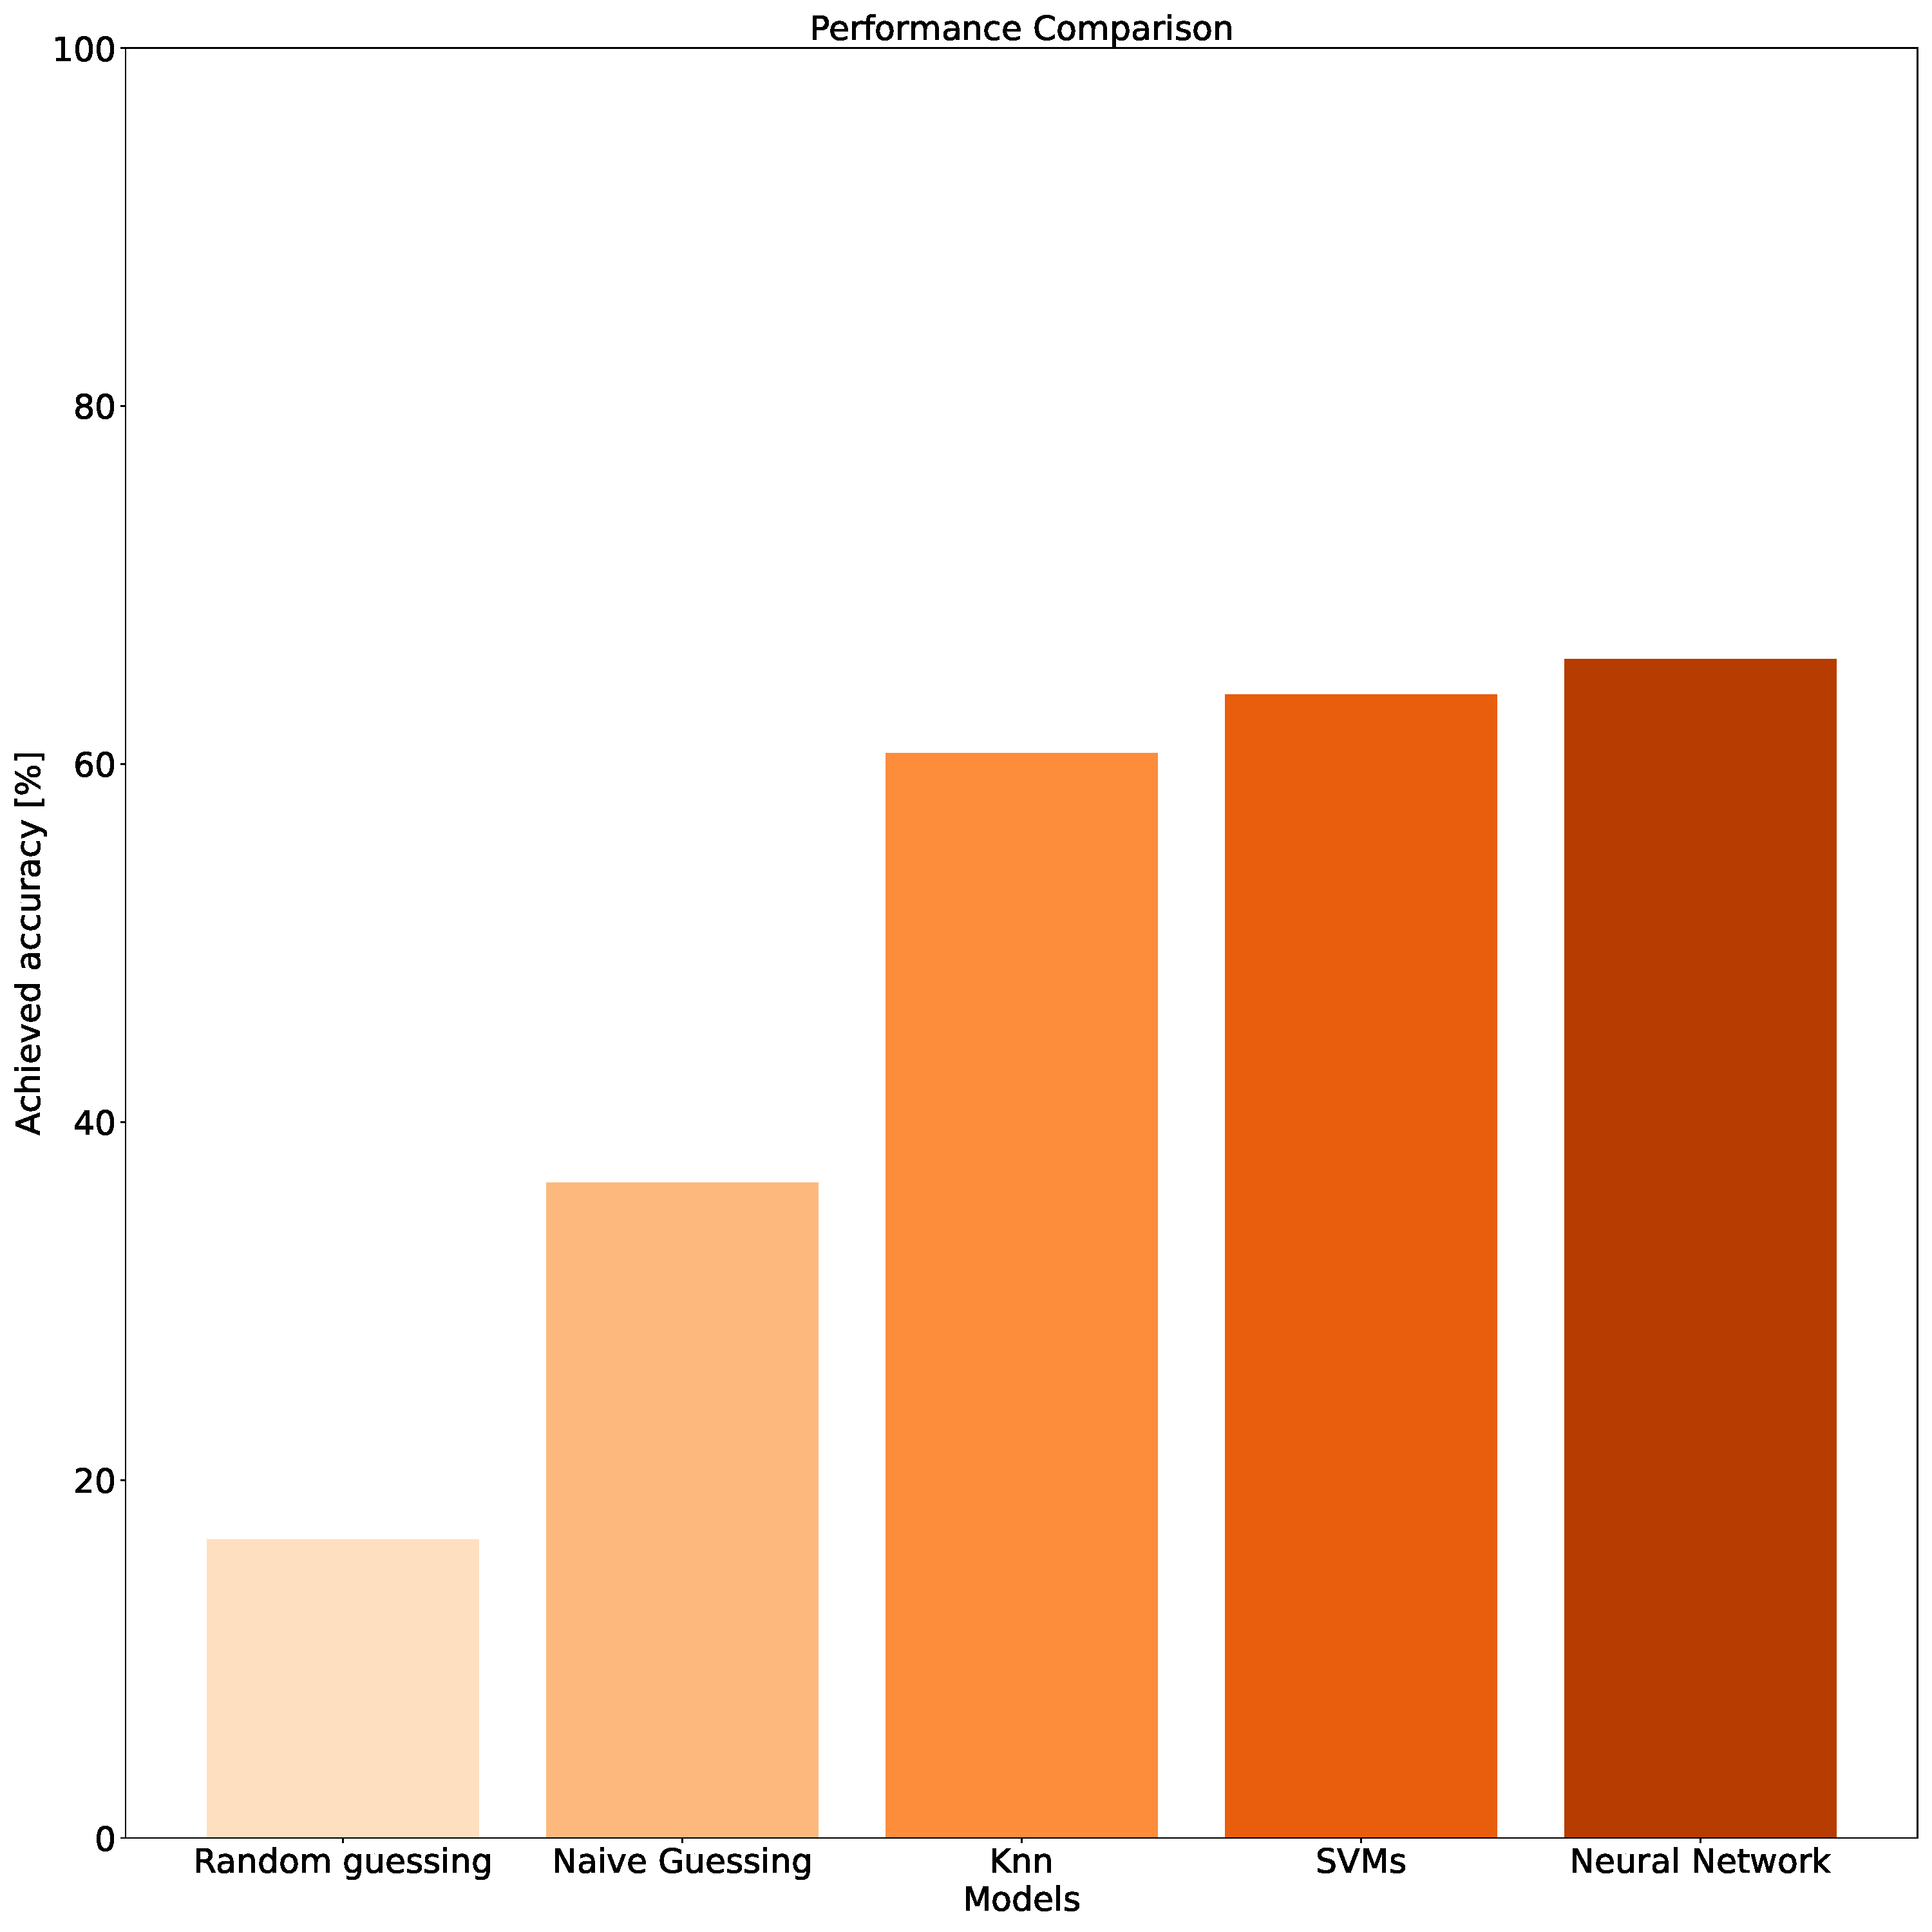
\includegraphics[scale=0.15]{figures/performance-comparison.pdf}
    % \caption{Comparison of the accuracy of different approaches.}
  \end{figure}
\end{frame}

% Alle Quellen, die bisher nicht zitiert wurden
%\nocite{Theories_of_grbs}

\printbibliography

\appendix
\begin{frame}
    \frametitle{Appendix: Accuracy and Loss}
    \begin{figure}
        \begin{minipage}[b]{0.48\textwidth}
            \centering
            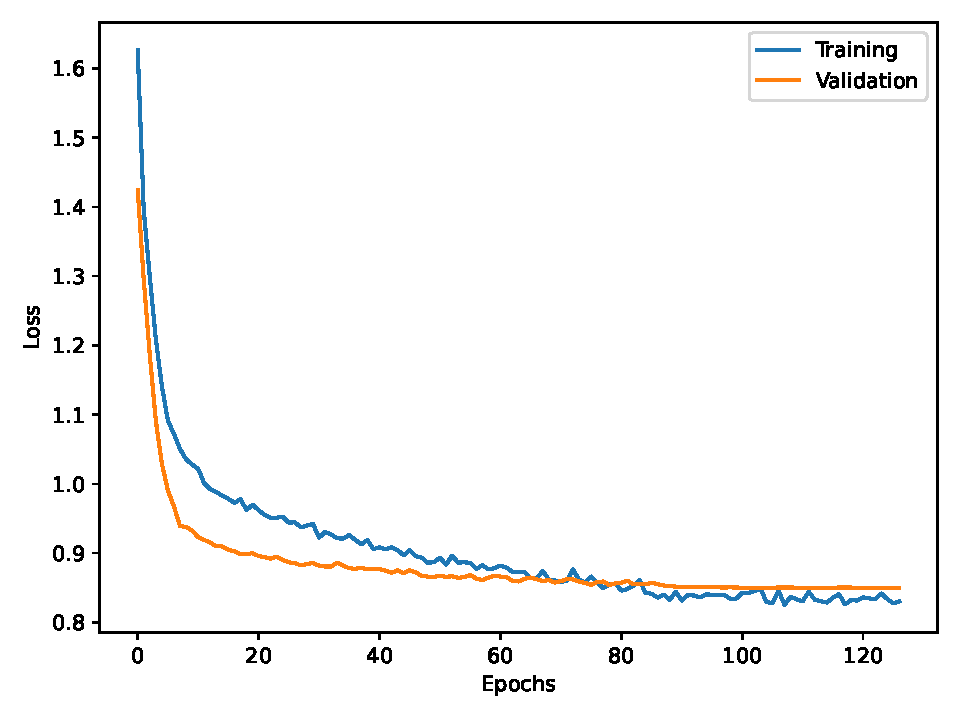
\includegraphics[width=\textwidth]{figures/Loss.pdf}
        \end{minipage}
        \hfill
        \begin{minipage}[b]{0.48\textwidth}
            \centering
            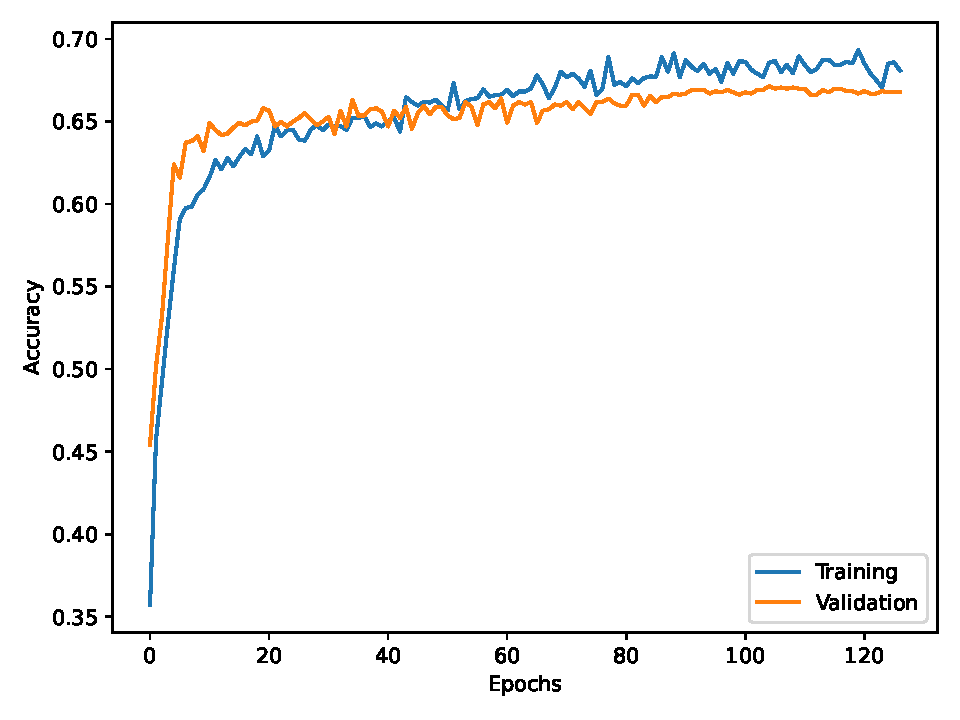
\includegraphics[width=\textwidth]{figures/Acc.pdf}
        \end{minipage}
    \end{figure}
\end{frame}
\begin{frame}
    \frametitle{Appendix: Precision-Recall Curve}
    \begin{figure}
        \begin{minipage}[b]{0.48\textwidth}
            \centering
            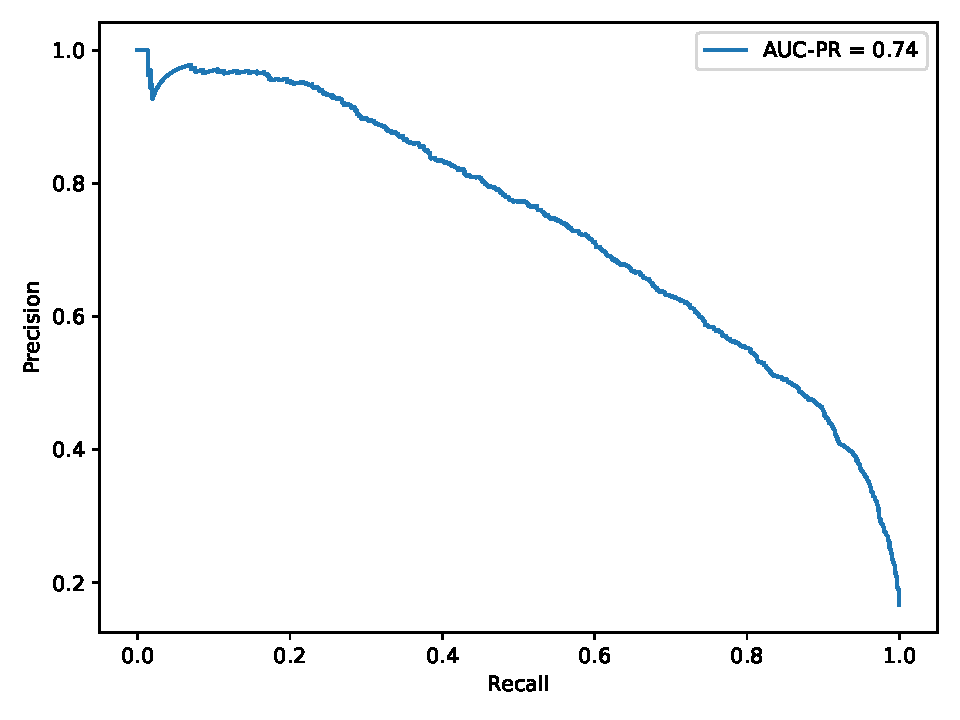
\includegraphics[width=\textwidth]{figures/PR_curve.pdf}
        \end{minipage}
        \hfill
        \begin{minipage}[b]{0.48\textwidth}
            \centering
            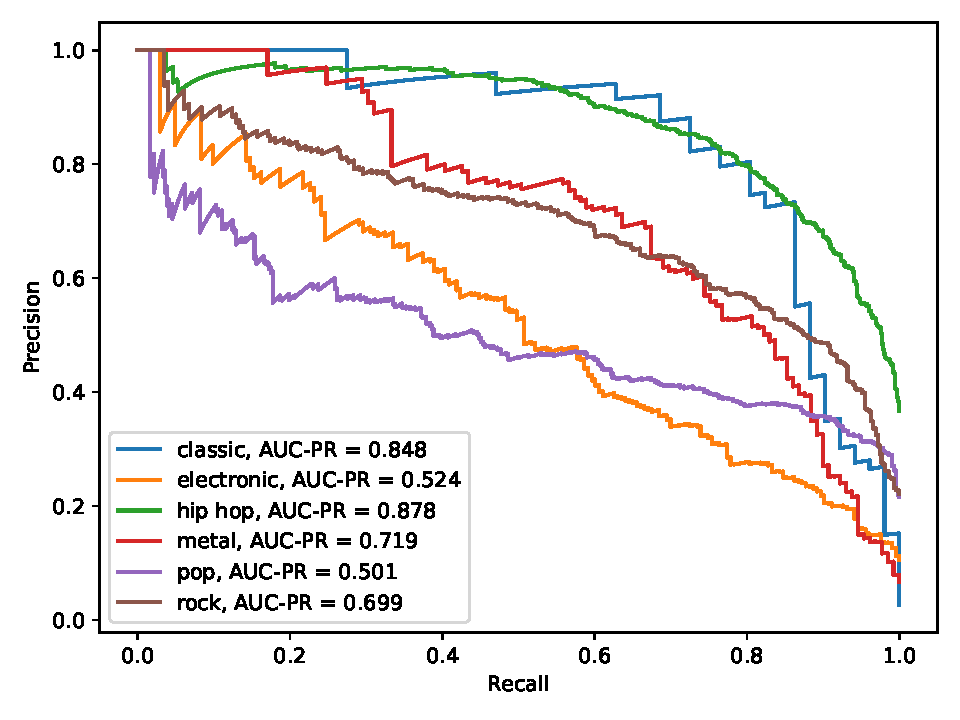
\includegraphics[width=\textwidth]{figures/PR_curve_genres.pdf}
        \end{minipage}
    \end{figure}
\end{frame}
\begin{frame}
    \frametitle{Appendix: Substructure of Hip Hop}
    \begin{figure}
        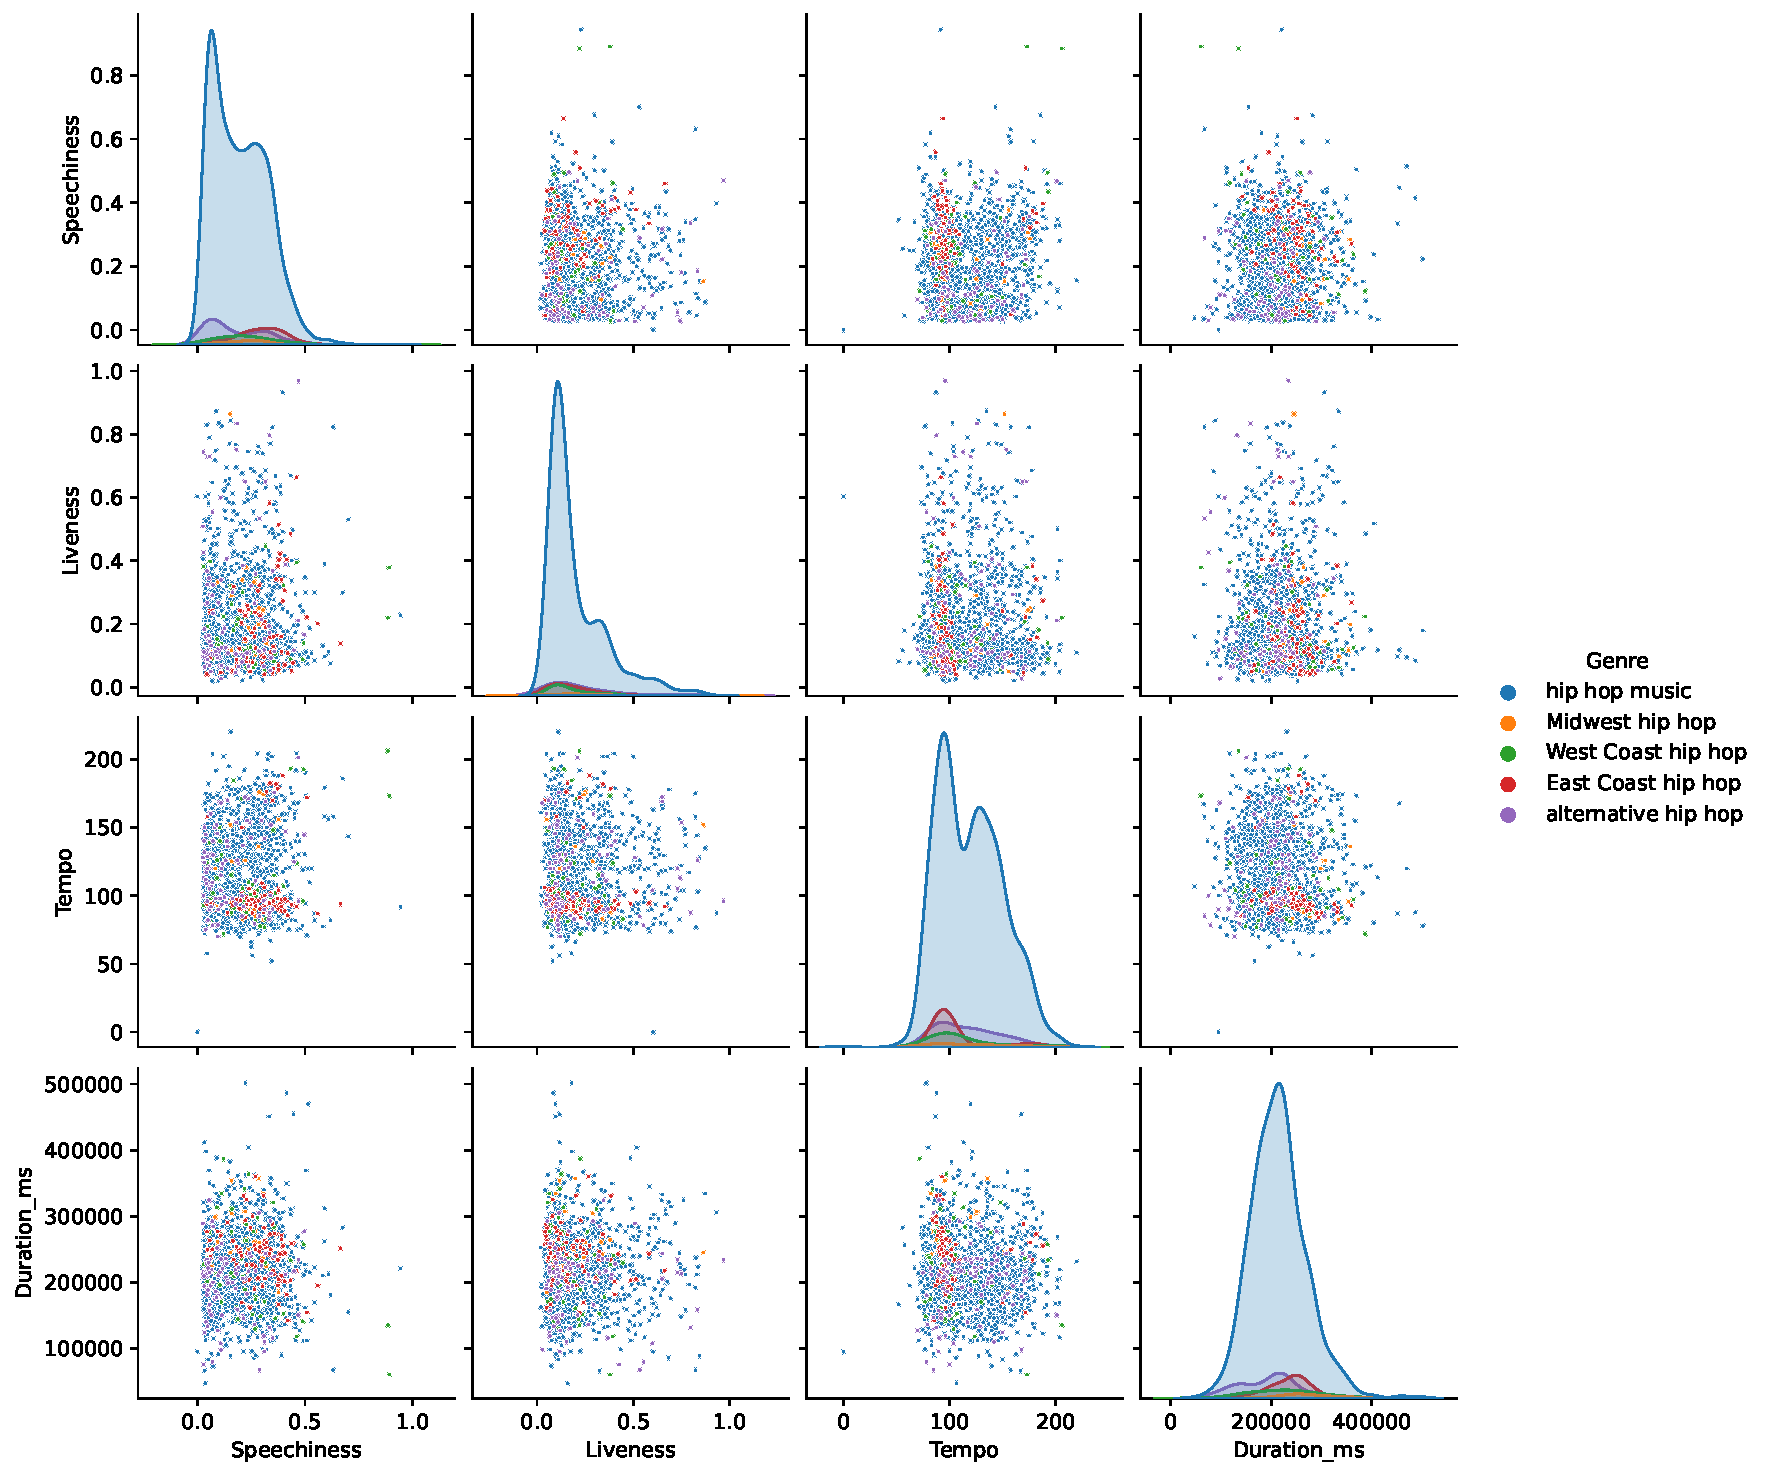
\includegraphics[scale=0.3]{figures/pairplot_hip_v3.pdf}
    \end{figure}
\end{frame}
\end{document}
